\chapter{Methods and Procedure}
\label{chapter:methods}

In figure \ref{fig:image}, the processing pipeline for this project is shown.

\begin{figure}[h!]
    \centering
    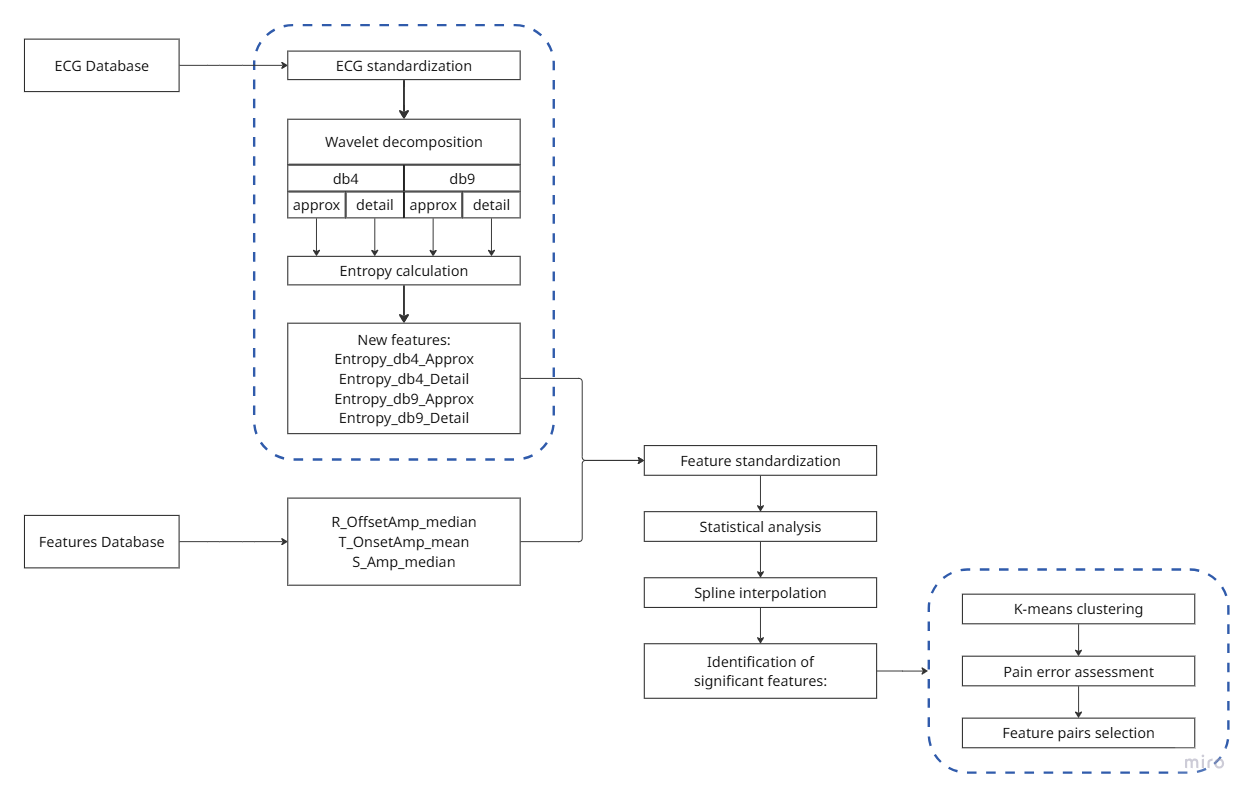
\includegraphics[width=1.0\textwidth]{image.png}
    \caption{Processing pipeline.}
    \label{fig:image}
\end{figure}

\section{Database Acquisition}
In this project, two databases were used: one has data from an \ac{ecg} signal while the other contains features extracted from that \ac{ecg}, as described in the article by Alves et al \cite{Alves2024}.

The data collection protocol followed a structured sequence designed to elicit and record both emotional and pain-related responses. It began with a 5-minute baseline period, during which participants remained seated in a relaxed position without any external stimuli. During this time, only physiological signals were recorded to establish a baseline.
Subsequently, participants watched a 10-minute video, composed of excerpts from comedy, horror, or documentary films, aimed at inducing positive, negative, or neutral emotional states, respectively. This was immediately followed by a second 5-minute stimulus-free period, allowing for recovery and stabilization of physiological responses.
Next, participants underwent a Cold Pressor Test (CPT), in which they immersed their non-dominant hand in a tank of cold water maintained at 7 ± 1°C. This procedure aimed to induce pain, and participants reported their experience using the Numerical Pain Scale (NPS) at four key time points: (1) before immersing the hand, (2) at the moment pain was first perceived (Pain Threshold), (3) when the pain became unbearable (Pain Tolerance), and (4) three minutes after hand removal. The CPT phase concluded either when the participant reached their pain tolerance or after a maximum of 2 minutes, whichever occurred first.
Finally, the protocol concluded with a third 5-minute period without stimuli, serving as a rest phase to observe post-task physiological responses. 
This process is depicted in figure \ref{fig:database}. 

(Referenciar todos os acrónimos?)

\begin{figure}[h!]
    \centering
    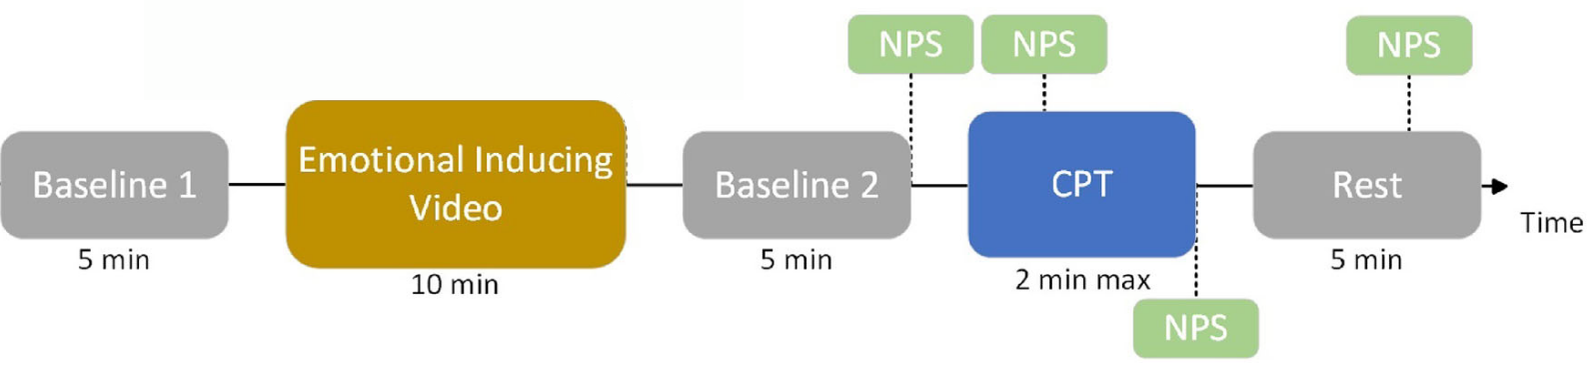
\includegraphics[width=1.0\textwidth]{database.png}
    \caption{Scheme of the protocol applied to obtain the database. (Adapted from \cite{Alves2024})}
    \label{fig:database}
\end{figure}

During the study, three physiological signals were recorded: electrocardiogram (ECG), electrodermal activity (EDA), and electromyography (EMG), with EMG signals collected specifically from the trapezius and triceps muscles. Among these, the ECG data were stored in a dedicated database, which was subsequently used in the present project.
From the ECG signals, several time series were extracted, including heart rate (HR), amplitude of wave peaks, amplitude of onsets and offsets, and the intervals between consecutive onsets, offsets, and peaks. These features were computed using 10-second sliding windows with a 50\% overlap.
For each window, a set of statistical metrics—namely the mean, median, and variance—was calculated, resulting in a total of 237 features. These were compiled into a features database, which was also employed in the current project.




\section{Feature Extraction}
Four of all the extrated features revealed to be more related to pain assessment, by the use of <diz o nome dos métodos que a Bruna usou para identificar as features mais importantes>. So, under the scope of this project, the median
of the R wave offset amplitude, the median of the T wave onset amplitude, and the mean and
median of the S wave peak amplitude were used as a base for subsequent analysis.
Considering that the previously described features are examples of the state of the art features in ECG analysis, and knowing that the pain quantification or identification is still an open area, this work wants to understand and find out other possible features that may describe the pain process. So, to accomplish such goal, an exploratory analysis to the collected ECG was performed.

% In the aforementioned article, the features of the ECG that can be used to best describe pain are defined.
% Hence, the top four features were selected for analysis, namely, the median of the R wave offset amplitude, the median of the T wave onset amplitude, and the mean and median of the S wave peak amplitude.

% To enhance this research, new features were sought out. For this reason, analysis of the ECG database itself was deemed necessary. 


\subsection{ECG Data Exploration}
When looking at the time series of the signal, in figure \ref{fig:ecg}, it's noticeable that the range of amplitudes of the QRS complex is way bigger than that of the P and T waves.
To tackle this, the ECG signal was standardized according to equation \ref{eq:1}, where X is the original ECG, $\mu$ is the mean, $\sigma$ is the standard deviation and Z is the standardized signal, which has mean zero and standard deviation one. 
This means the range of values is the same for all participants, reducing the intervariability that is induced by the initial state of the participant, since it is an uncontrolled variable.

\begin{equation} \label{eq:1}
Z = \frac{X-\mu}{\sigma}
\end{equation}

% \begin{figure}[h!]
%     \centering
%     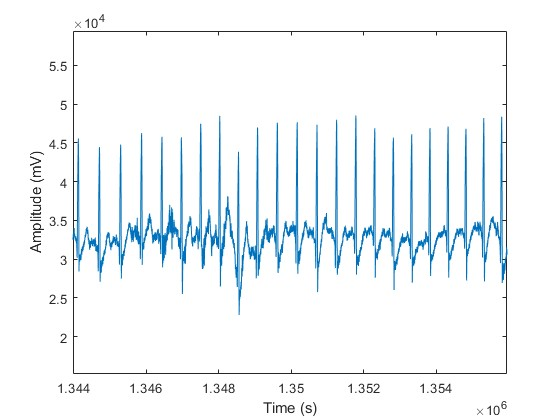
\includegraphics[width=0.9\textwidth]{ecg.jpg}
%     \caption{Section of the ECG signal of a participant.}
%     \label{fig:ecg}
% \end{figure}

\begin{figure}[htbp]
    \centering
    \begin{minipage}{0.45\textwidth}
        \centering
        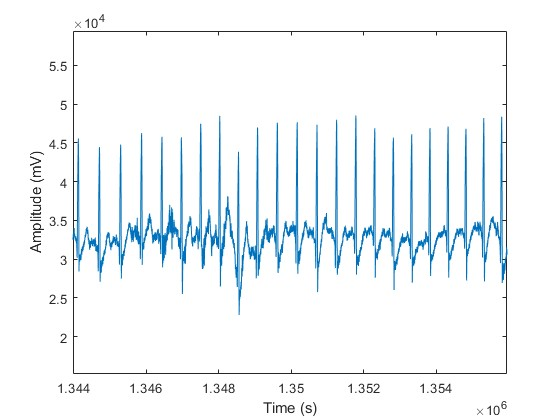
\includegraphics[width=6.5cm]{ecg}
        \caption{Section of the ECG signal of a participant.}
        \label{fig:ecg}
    \end{minipage}
    \hfill
    \begin{minipage}{0.45\textwidth}
        \centering
        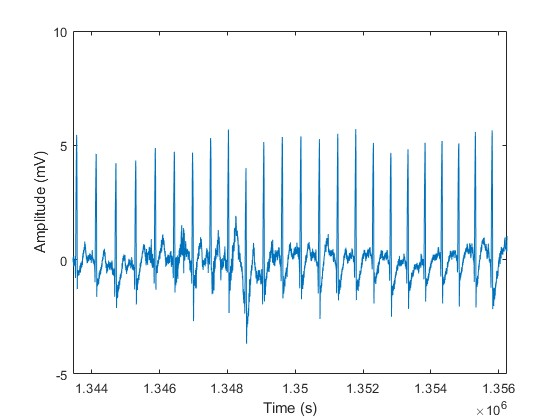
\includegraphics[width=6.5cm]{normalized ecg}
        \caption{Section of the standardized ECG signal of a participant.}
        \label{fig:normalized_ecg}
    \end{minipage}
\end{figure}

Once the signal was standardized, fluctuations were noticed in the time series.
By removing high frequencies from the signal, by filtering for example, these would be alleviated.
However, there could be information related to pain associated to those frequencies.
%The solution to solve both of these problems was to decompose the signal in wavelets. 

(Falar das famílias de wavelets para análise de ECGs?)

To choose the best type of wavelet, two criteria were established: one's format should be similar to that of the ECG wave and the other should have a higher frequency, while still maintaining its smoothness.
Accordingly, Daubechies-4 ('db4') and Daubechies-9 ('db9') were chosen.
Regarding the number of levels of decomposition, as can be seen in figure \ref{fig:wavelets2}, when there are two levels the R peak is noticeable in the first detail, which is not something this project means to highlight.
Therefore, only one level of decomposition was applied.

\begin{figure}[h!]
    \centering
    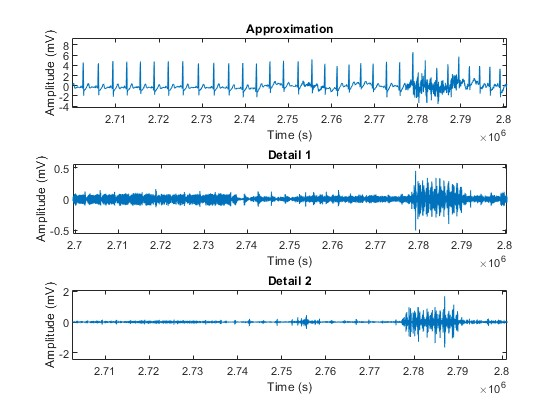
\includegraphics[width=0.8\textwidth]{wavelets 2.jpg}
    \caption{Daubechies-4 Wavelet Decomposition - level 2.}
    \label{fig:wavelets2}
\end{figure}


\subsection{Entropy Calculation}
Entropy quantifies the order or disorder of information that a signal presents. Since this quantity might be affected in the ECG when someone feels pain, it was extracted from the resulting wavelets, functioning as a new feature. In order to keep consistency with the other features, a same sized window was used, that is, 10 seconds with 50\% overlap. 

(Justificar tipo de entropia que escolhi? - approximation)




\section{Data Analysis}
To do the optimal processing of the features, fifteen participants were selected at random. After standardizing the features, so that they're comparable with each other, graphics of the time series of the features were plotted for each participant. An example can be seen in figure \ref{fig:featurestimeseries}, in which a clear change can be seen when the participant dips their hand in water, feeling pain. Since the timeseries of the mean and median of the S wave amplitude were so similar, it was decided that only the median would be analysed.

(Falta ajustar imagem para eixo do y não ficar sobreposto.)

\begin{figure}[htbp]
    \centering
    \begin{minipage}{0.48\textwidth}
        \centering
        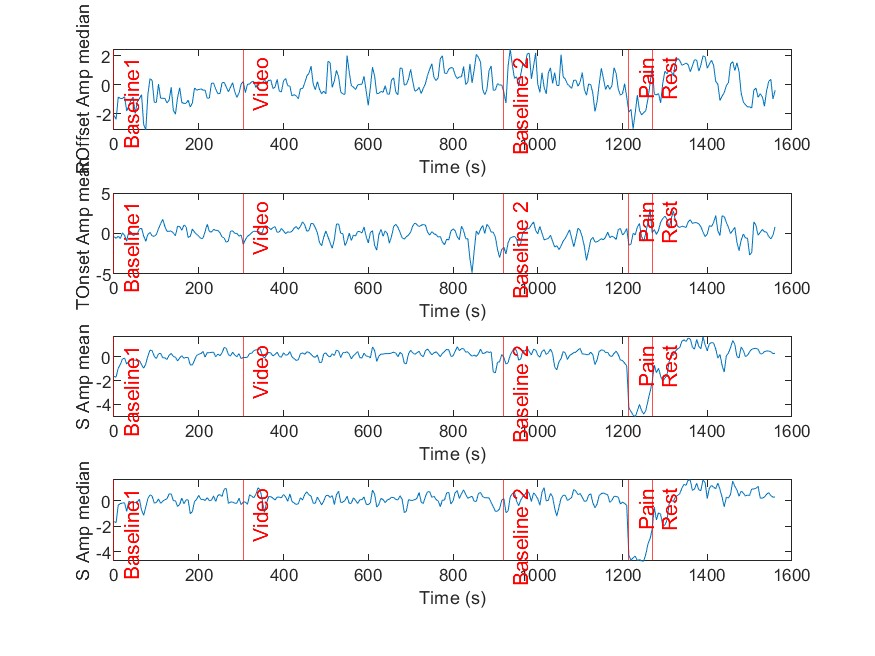
\includegraphics[width=\linewidth]{orig_part5.jpg}
    \end{minipage}
    \hspace{0.005\textwidth} % pequeno espaço entre as imagens
    \begin{minipage}{0.48\textwidth}
        \centering
        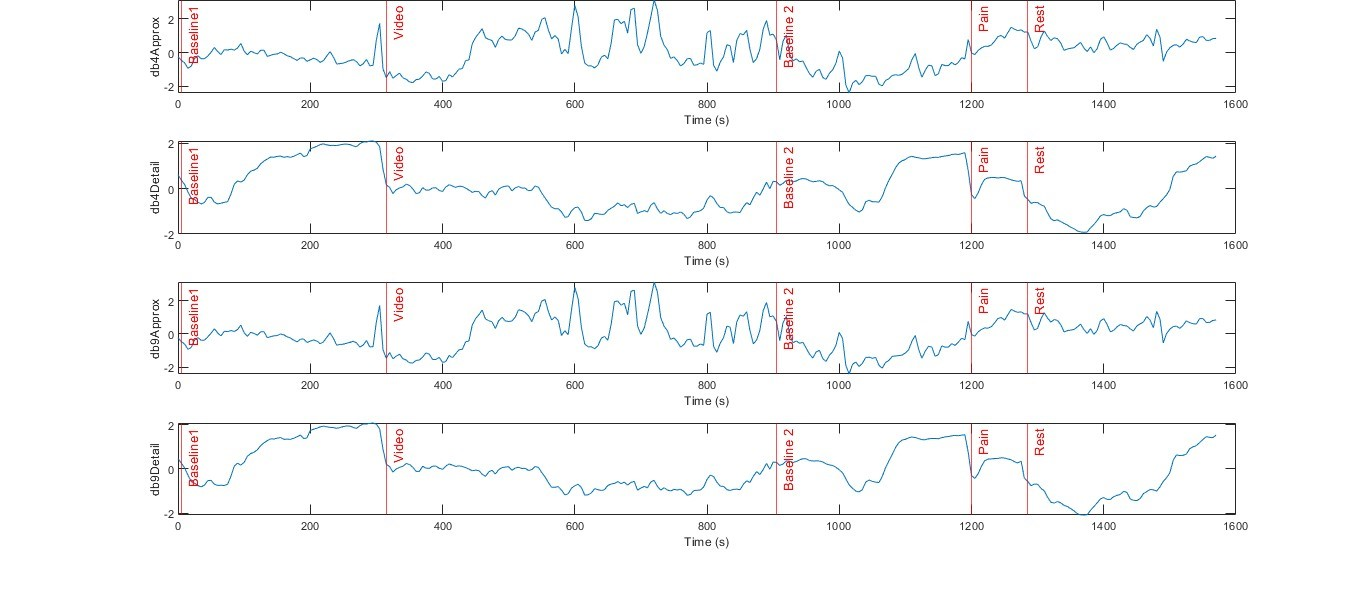
\includegraphics[width=\linewidth]{entropy_part5.jpg}
    \end{minipage}
    \caption{Standardized features' time series.}
    \label{fig:featurestimeseries}
\end{figure}

Subsequently, a statistical analysis of the participants’ features was conducted using histograms, as illustrated in Figure \ref{fig:histogram}. The histograms revealed that the distributions of the features deviate from normality, justifying the use of the median and interquartile range (IQR) as measures of central tendency and dispersion, respectively.
These values were computed for each feature and considered as derived features that will integrate the analysis.

\begin{figure}[h!]
    \centering
    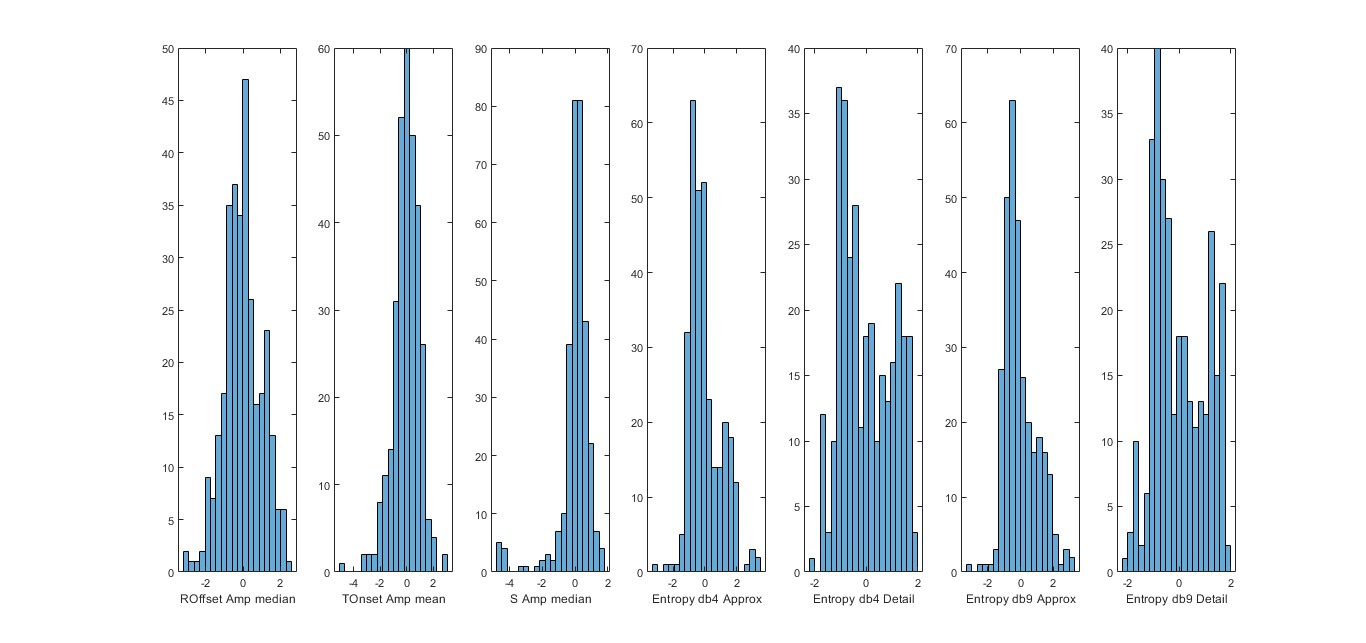
\includegraphics[width=0.8\textwidth]{histogram.jpg}
    \caption{Histograms of the features.}
    \label{fig:histogram}
\end{figure}

The goal of this project is to select features that distinguish pain from no pain. To do this, it’s important to guarantee the synchronization between segments, so that they’re comparable. To accomplish this goal, spline interpolation was done in each step, conducing to equalize the number of points to a 60 seconds intervals. The result of this method is portrayed in figure \ref{fig:normalizedfeatures}. 

\begin{figure}[h!]
    \centering
    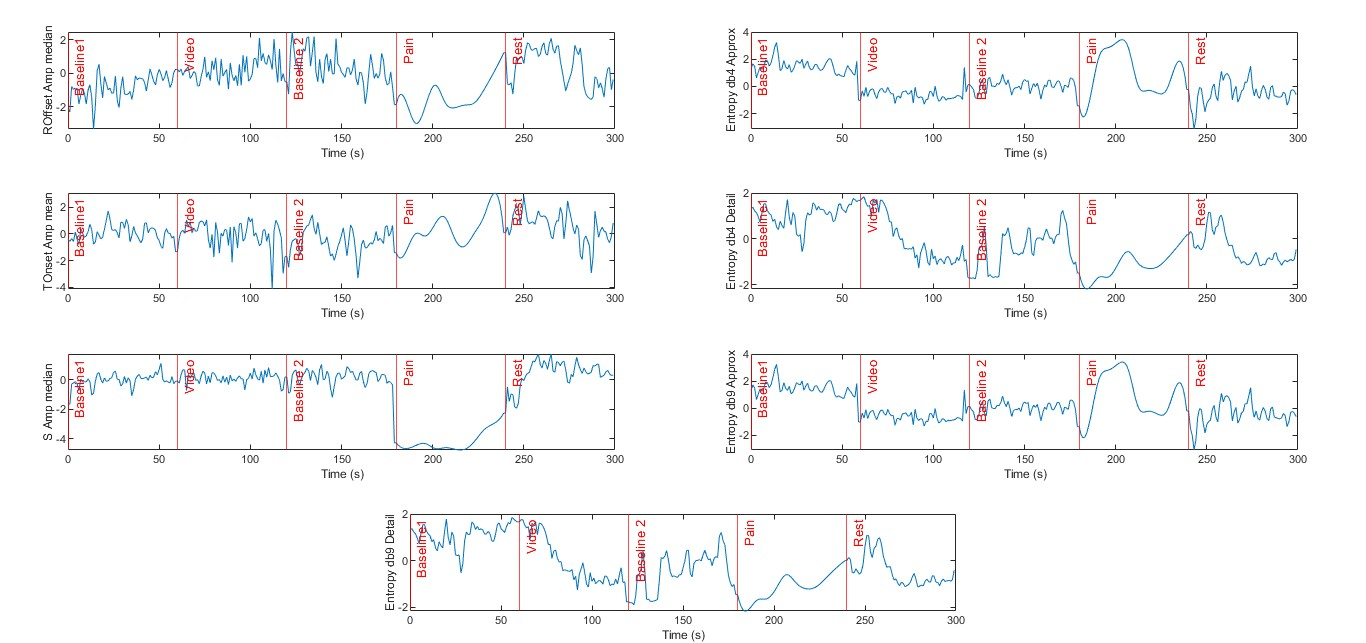
\includegraphics[width=1\textwidth]{normalized features.jpg}
    \caption{Features normalized in time after interpolation.}
    \label{fig:normalizedfeatures}
\end{figure}









